\documentclass[journal]{IEEEtran}

\usepackage{amsmath,amssymb,amsfonts,mathtools}
\usepackage[T1]{fontenc}
\usepackage{booktabs}
\usepackage{graphicx}
\usepackage{multirow}
\usepackage{url}
\usepackage{cite}
\usepackage{xr}
\externaldocument{main}

\renewcommand{\thetable}{S\arabic{table}}
\renewcommand{\thefigure}{S\arabic{figure}}

\begin{document}

\title{Supplementary Material for\\
SynAP-Fib: Synergistic Anatomical Priors for Fine-Grained Ultrasound
Liver Fibrosis Grading in Schistosomiasis}

\author{Ziyang~Xu, \textit{et al.}}

\maketitle

All results below are computed on the patient-held-out test set (4,107 images,
240 patients, 4 centers) using each configuration's validation-selected
checkpoint under the single prespecified seed~2026. Configuration A is the
SFibAI baseline, B the letterbox control, C position-only, D lesion-only, and
E the joint configuration (SynAP-Fib).

\section{Per-Center Descriptive Performance}

\begin{figure}[!htbp]
\centering
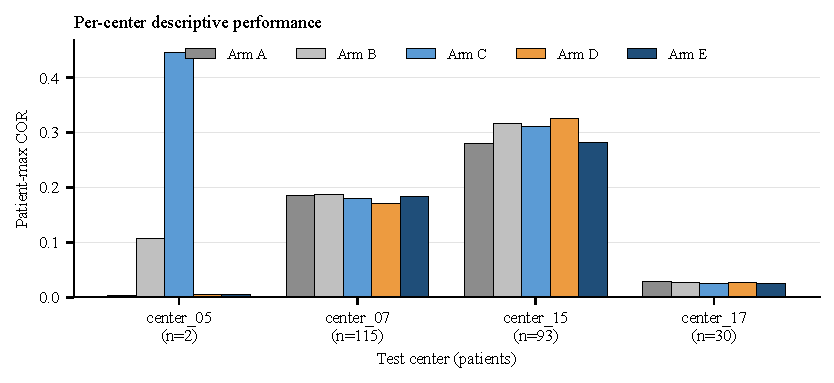
\includegraphics[width=0.86\columnwidth]{figures/supp_fig_s1.pdf}
\caption{Per-center descriptive performance on the patient-held-out test set.
All test centers were represented in the training split; therefore, these
results characterize center-wise performance heterogeneity rather than
generalization to unseen centers. Axis labels carry patient counts.
Estimates from centers contributing few patients are descriptive and should be
interpreted with caution. The same values are tabulated in
Table~\ref{tab:percenter}.}
\label{fig:suppcenter}
\end{figure}

\section{Error Distribution Analysis}

\begin{figure}[!htbp]
\centering
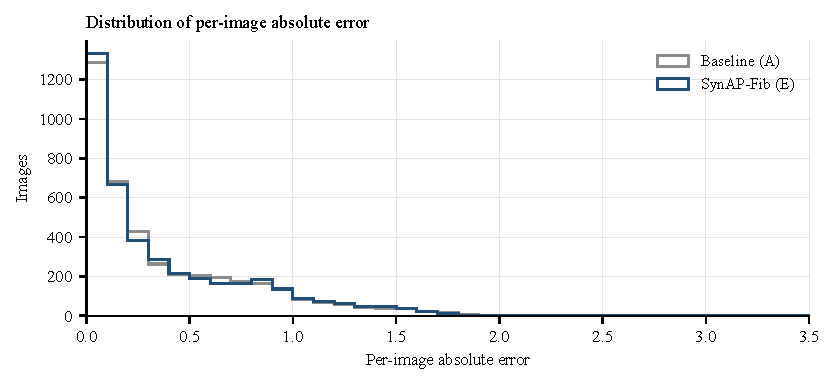
\includegraphics[width=0.86\columnwidth]{figures/supp_fig_s2.pdf}
\caption{Distribution of per-image absolute error on the patient-held-out test
set, arms A and E (4,107 images each), computed from the frozen per-image
predictions.}
\label{fig:supperr}
\end{figure}

\section{Training and Checkpoint-Selection Trajectories}

\begin{figure}[!htbp]
\centering
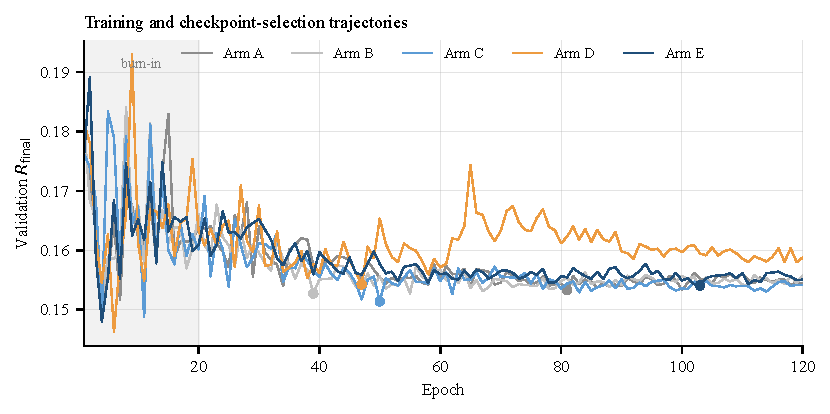
\includegraphics[width=0.86\columnwidth]{figures/supp_fig_s3.pdf}
\caption{Per-epoch validation $R_{\mathrm{final}}$ for all five
configurations (epochs 1--120, no smoothing). Markers indicate the
validation-selected checkpoint of each configuration; epochs 1--20 are
burn-in and ineligible for selection. The test set plays no role in
checkpoint selection.}
\label{fig:supptraj}
\end{figure}

\section{Paired Bootstrap Analysis of Prespecified Contrasts}

Table~\ref{tab:boot} reports the prespecified contrasts under
10,000 center-stratified, patient-cluster paired bootstrap replicates. All
configurations share the same patient resampling draws, so contrasts are paired.
Confidence intervals are percentile intervals.

A negative delta favours the candidate configuration, since lower
$R_{\mathrm{final}}$ is better.

\begin{table*}[!t]
\centering
\caption{Paired bootstrap analysis of the prespecified contrasts on
$R_{\mathrm{final}}$. $P$ denotes the proportion of bootstrap replicates in
which the candidate achieved a lower $R_{\mathrm{final}}$; \textbf{it is not a
frequentist $p$-value}. Negative deltas favour the candidate.}
\label{tab:boot}
\footnotesize
\setlength{\tabcolsep}{3pt}
\begin{tabular}{@{}l rrr r@{}}
\toprule
Contrast & Observed $\Delta$ & Mean $\pm$ SD & 95\% CI & $P$ \\
\midrule
A $-$ B & $-0.010789$ & $-0.010804 \pm 0.005689$ & $[-0.021909, +0.000310]$ & 0.971 \\
C $-$ A & $+0.012890$ & $+0.012920 \pm 0.005234$ & $[+0.002762, +0.023122]$ & 0.007 \\
D $-$ A & $+0.009374$ & $+0.009370 \pm 0.005784$ & $[-0.001717, +0.020827]$ & 0.052 \\
E $-$ A & $-0.000447$ & $-0.000447 \pm 0.006116$ & $[-0.012287, +0.011826]$ & 0.533 \\
E $-$ C & $-0.013337$ & $-0.013367 \pm 0.005631$ & $[-0.024376, -0.002223]$ & 0.990 \\
E $-$ D & $-0.009821$ & $-0.009817 \pm 0.005542$ & $[-0.020718, +0.001010]$ & 0.961 \\
\bottomrule
\end{tabular}
\end{table*}

The E $-$ A interval spans zero: on the primary endpoint the
joint configuration and the baseline are not distinguishable under this
analysis. We therefore describe E as the best observed configuration and do not
claim an improvement over the baseline. The C $-$ A and E $-$ C intervals
exclude zero.

\section{Discrimination and Calibration}

\begin{table}[!t]
\centering
\caption{Image-level discrimination and calibration. Lower is better for the
Brier score and expected calibration error (ECE).}
\label{tab:auc}
\footnotesize
\setlength{\tabcolsep}{4pt}
\begin{tabular}{@{}l rrrr@{}}
\toprule
Arm & Macro AUROC~$\uparrow$ & Macro AUPRC~$\uparrow$ & Brier~$\downarrow$ & ECE~$\downarrow$ \\
\midrule
A & 0.888217 & 0.718714 & 0.493755 & 0.175061 \\
B & 0.887697 & 0.724624 & 0.485416 & 0.170211 \\
C & 0.884395 & 0.711592 & 0.503889 & 0.183766 \\
D & 0.879815 & 0.706133 & 0.519752 & 0.188694 \\
E & \textbf{0.891698} & \textbf{0.729264} & \textbf{0.474036} & \textbf{0.164196} \\
\bottomrule
\end{tabular}
\end{table}

\section{Patient-Median Aggregation}

Patient-median aggregation is a robustness analysis; patient-max is the
prespecified patient-level aggregation and is reported in the main text.

\begin{table}[!t]
\centering
\caption{Patient-median clinical objective risk. Lower is better.}
\label{tab:pmed}
\small
\begin{tabular}{@{}l r@{}}
\toprule
Arm & Patient-median COR~$\downarrow$ \\
\midrule
A & 0.163623 \\
B & 0.159540 \\
C & 0.168302 \\
D & 0.167317 \\
E & \textbf{0.154344} \\
\bottomrule
\end{tabular}
\end{table}

\section{Center-Balanced Aggregation and Per-Center Results}

\begin{table}[!t]
\centering
\caption{Center-balanced patient-max clinical objective risk, aggregated with
weights proportional to the square root of each center's patient count. Lower is
better.}
\label{tab:cb}
\small
\begin{tabular}{@{}l r@{}}
\toprule
Arm & Center-balanced patient-max COR~$\downarrow$ \\
\midrule
A & 0.177622 \\
B & 0.196765 \\
C & 0.209305 \\
D & 0.188052 \\
E & \textbf{0.177453} \\
\bottomrule
\end{tabular}
\end{table}

\begin{table}[!t]
\centering
\caption{Per-center descriptive performance on the patient-held-out test set.
All test centers were represented in the training split; therefore, these
results characterize center-wise performance heterogeneity rather than
generalization to unseen centers. Estimates from centers contributing few
patients are descriptive and should be interpreted with caution.}
\label{tab:percenter}
\footnotesize
\setlength{\tabcolsep}{3.5pt}
\begin{tabular}{@{}l r rrrrr@{}}
\toprule
Center & $n$ & A & B & C & D & E \\
\midrule
center\_05 &   2 & 0.003978 & 0.106383 & 0.445622 & 0.004904 & 0.005329 \\
center\_07 & 115 & 0.184925 & 0.188137 & 0.180888 & 0.170010 & 0.183879 \\
center\_15 &  93 & 0.279634 & 0.316480 & 0.310589 & 0.326305 & 0.281672 \\
center\_17 &  30 & 0.028546 & 0.026213 & 0.025597 & 0.027244 & 0.025816 \\
\bottomrule
\end{tabular}
\end{table}

\section{Post-Hoc Ordinal Agreement}

Quadratic-weighted Cohen's $\kappa$ was recomputed post hoc from the frozen
per-image predictions and is not a prespecified endpoint. Continuous
posterior-expectation predictions were mapped to the nearest one of the 36 valid
grades before computing $\kappa$; posterior argmax predictions were not used.

\begin{table}[!t]
\centering
\caption{Post-hoc 36-level quadratic-weighted Cohen's $\kappa$ at the image
level. Higher is better.}
\label{tab:qwk}
\small
\begin{tabular}{@{}l r@{}}
\toprule
Arm & QWK~$\uparrow$ \\
\midrule
A & 0.864009 \\
B & 0.857924 \\
C & 0.861988 \\
D & 0.854622 \\
E & \textbf{0.864566} \\
\bottomrule
\end{tabular}
\end{table}

\section{Auxiliary Branch Details}

\begin{table}[!t]
\centering
\caption{Per-class recall of the six-class anatomical position head.}
\label{tab:posrec}
\small
\begin{tabular}{@{}l rrrrrr@{}}
\toprule
Arm & p1 & p2 & p3 & p4 & p5 & p6 \\
\midrule
C & 0.8141 & 0.6309 & 0.5327 & 0.5618 & 0.6569 & 0.7872 \\
E & 0.8473 & 0.6509 & 0.5457 & 0.5261 & 0.6686 & 0.7679 \\
\bottomrule
\end{tabular}
\end{table}

\begin{table}[!t]
\centering
\caption{Learned gate distributions for the anatomical residual pathways,
reported as a mechanistic diagnostic. Gate values remained above zero rather
than collapsing. Gate magnitude alone does not quantify how much a branch
contributed, because the effective contribution also depends on residual
feature magnitude.}
\label{tab:gates}
\footnotesize
\setlength{\tabcolsep}{3.5pt}
\begin{tabular}{@{}ll rrrrr@{}}
\toprule
Arm & Branch & Mean & SD & P10 & P50 & P90 \\
\midrule
C & Position & 0.097689 & 0.011298 & 0.086365 & 0.094788 & 0.114185 \\
D & Lesion   & 0.002344 & 0.003434 & 0.001769 & 0.002234 & 0.002876 \\
E & Position & 0.084124 & 0.011330 & 0.072815 & 0.080933 & 0.101379 \\
E & Lesion   & 0.006513 & 0.017638 & 0.003479 & 0.004543 & 0.006386 \\
\bottomrule
\end{tabular}
\end{table}

\section{Unrounded Computational Cost}

Table~\ref{tab:cost} gives the unrounded values summarized in the main text.
Measurements use batch~1 on $3\times512\times512$ input, counting Conv2d and
Linear operations only at two FLOPs per multiply--accumulate, under CUDA
automatic mixed precision in eager mode with 10 warmup and 30 measured
iterations.

\begin{table}[!t]
\centering
\caption{Unrounded parameter counts, arithmetic cost and latency.}
\label{tab:cost}
\footnotesize
\setlength{\tabcolsep}{3.5pt}
\begin{tabular}{@{}l rrrr@{}}
\toprule
Arm & Parameters & GFLOPs & Latency med.~(ms) & Latency P90 (ms) \\
\midrule
A & 24,579,684 & 42.709 & 3.031 & 3.356 \\
B & 24,579,684 & 42.709 & 2.989 & 3.350 \\
C & 24,610,739 & 42.709 & 3.521 & 4.010 \\
D & 25,991,302 & 43.918 & 3.607 & 4.245 \\
E & 26,022,357 & 43.918 & 3.993 & 4.427 \\
\bottomrule
\end{tabular}
\end{table}

Table~\ref{tab:unroundaux} gives the auxiliary branch metrics of the main-text
Table~IV at their recorded precision; the main table displays these values
rounded to four decimal places.

\begin{table}[!t]
\centering
\caption{Auxiliary branch metrics at recorded precision (the main-text
Table~IV displays four decimal places). Position metrics cover the six-class
anatomical protocol; lesion metrics are weak-box agreement, not segmentation
ground truth.}
\label{tab:unroundaux}
\footnotesize
\setlength{\tabcolsep}{3pt}
\begin{tabular}{@{}l rrr rr@{}}
\toprule
 & \multicolumn{3}{c}{Position branch} & \multicolumn{2}{c}{Weak-box} \\
\cmidrule(lr){2-4} \cmidrule(lr){5-6}
Arm & Acc. & Macro-F1 & CE & Dice@0.5 & IoU@0.5 \\
\midrule
C & 66.40\% & 0.662250 & 0.944391 & -- & -- \\
D & -- & -- & -- & 0.353920 & 0.226066 \\
E & 66.81\% & 0.665861 & 0.916542 & 0.360312 & 0.235487 \\
\bottomrule
\end{tabular}
\end{table}

\section{Stage-Wise Mean Absolute Error}

Stage-wise mean absolute error was recomputed post hoc from the frozen per-image
predictions, grouped by true grade. Figure~\ref{fig:stagewise} of the main text
plots configurations A and E; all five are given here for completeness.

\begin{table}[!t]
\centering
\caption{Post-hoc stage-wise mean absolute error by true grade. Support:
F0 $n=1140$, F1 $n=1006$, F2 $n=1108$, F3 $n=853$, identical for all
configurations. Lower is better.}
\label{tab:stagemae}
\small
\begin{tabular}{@{}l rrrr@{}}
\toprule
Arm & F0 & F1 & F2 & F3 \\
\midrule
A & 0.196508 & 0.416107 & 0.514474 & 0.403570 \\
B & 0.215458 & 0.387597 & 0.496175 & 0.451800 \\
C & 0.215293 & 0.394219 & 0.510325 & 0.423316 \\
D & 0.223659 & 0.416849 & 0.517423 & 0.426352 \\
E & 0.196277 & 0.411035 & 0.516525 & 0.401280 \\
\bottomrule
\end{tabular}
\end{table}

\begin{table}[!t]
\centering
\caption{Stage-wise recall of the four clinical grades. Higher is better.}
\label{tab:stagerec}
\small
\begin{tabular}{@{}l rrrr@{}}
\toprule
Arm & F0 & F1 & F2 & F3 \\
\midrule
A & 80.18\% & 49.50\% & 63.63\% & 73.27\% \\
B & 77.37\% & 55.47\% & 65.79\% & 70.22\% \\
C & 76.32\% & 53.38\% & 62.91\% & 70.57\% \\
D & 77.63\% & 46.92\% & 60.65\% & 71.40\% \\
E & 81.14\% & 50.50\% & 63.63\% & 72.10\% \\
\bottomrule
\end{tabular}
\end{table}

\section{Additional Image-Level Error Profile}

\begin{table}[!t]
\centering
\caption{Image-level error profile. TMAE is the excess-error metric beyond a
$0.5$ tolerance; the severe error rate is defined on the continuous score as
$\Pr(|\hat{y}-y| > 1.0)$. Lower is better for both, and for MAE.}
\label{tab:errprof}
\small
\begin{tabular}{@{}l rrrr@{}}
\toprule
Arm & MAE~$\downarrow$ & $\pm0.3$ acc.~$\uparrow$ & TMAE~$\downarrow$ & Severe error~$\downarrow$ \\
\midrule
A & 0.379086 & 58.29\% & 0.122417 & 9.08\% \\
B & 0.382443 & 57.78\% & 0.123630 & 9.59\% \\
C & 0.381920 & 56.15\% & \textbf{0.121283} & 9.50\% \\
D & 0.392331 & 57.12\% & 0.131776 & 10.37\% \\
E & \textbf{0.377857} & 57.95\% & 0.123100 & 9.37\% \\
\bottomrule
\end{tabular}
\end{table}

\end{document}
